\begin{figure}[pos=p]
\begin{center}
\begin{overpic}[width=0.48\textwidth]{img/results_lrt_05261515_135_12.pdf}%
\put(690,250){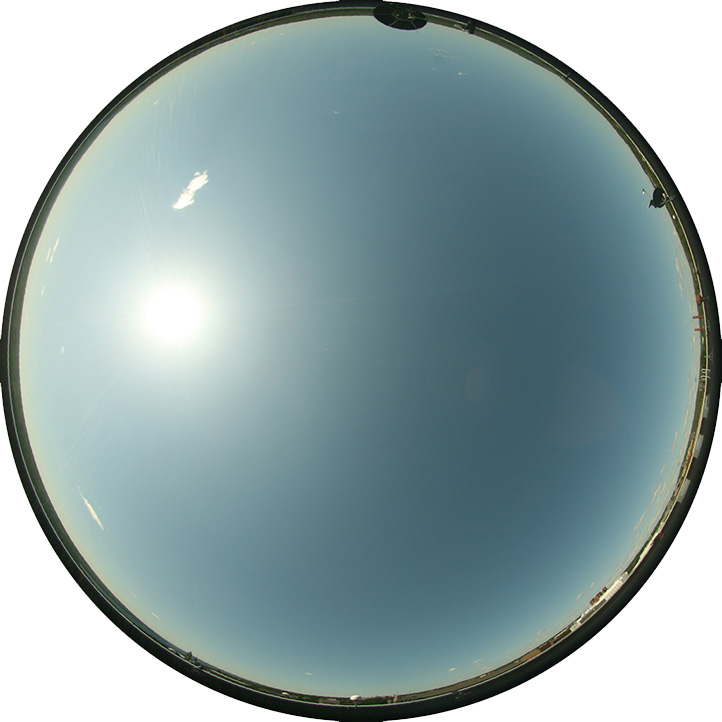
\includegraphics[width=0.125\textwidth]{img/05261515.jpg}}%
\put(905,455){\linethickness{0.4mm}\color{yellow}\circle{40}}%
\end{overpic}%
~%
\begin{overpic}[width=0.48\textwidth]{img/results_lrt_05271015_135_12.pdf}%
\put(690,250){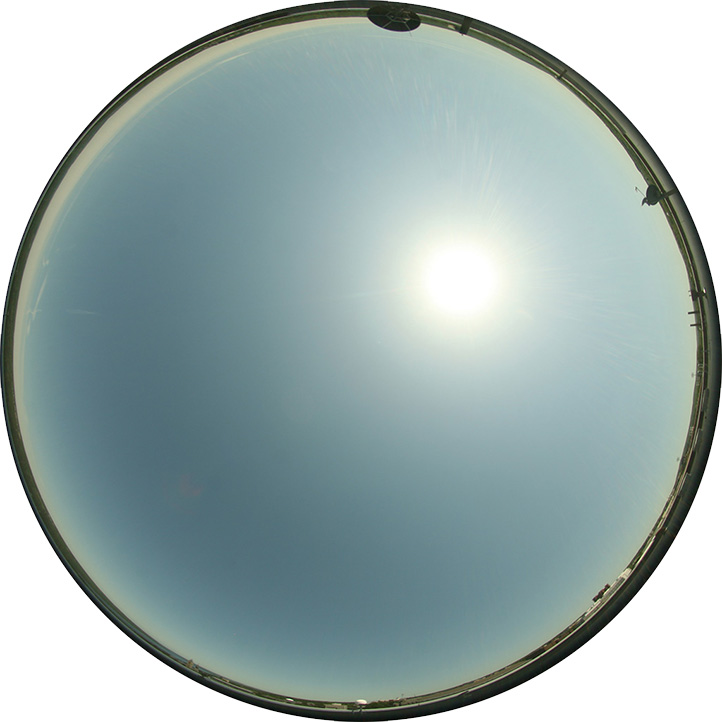
\includegraphics[width=0.125\textwidth]{img/05271015.jpg}}%
\put(905,455){\linethickness{0.4mm}\color{yellow}\circle{40}}%
\end{overpic}%
% ~%
% \begin{overpic}[width=0.325\textwidth]{img/results_lrt_09241539_135_12.pdf}%
% \put(690,250){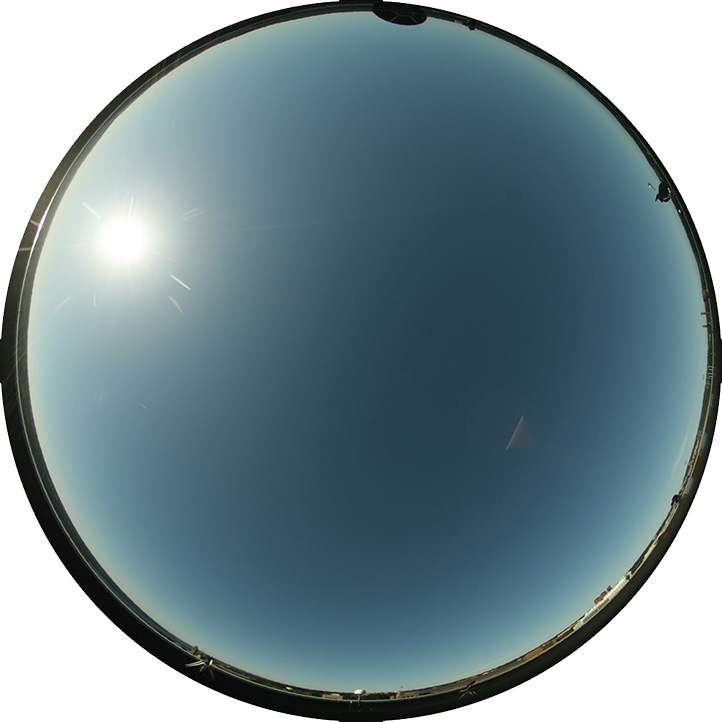
\includegraphics[width=0.09\textwidth]{img/09241539.jpg}}%
% \put(920,470){\linethickness{0.3mm}\color{blue}\circle{35}}%
% \end{overpic}%
%\vspace{-2mm}
\caption[lrt3312]{Spectral radiance at (33.75\degree~azimuth, 12.12\degree~altitude), circled, for two of the holdout test skies in \autoref{tab:testskies}. Spectroradiometer measurement, ETR model prediction, and libRadtran estimation plotted.}
\label{fig:lrt_3312}
\end{center}
\end{figure}

\begin{figure}[pos=p]
\begin{center}
\begin{overpic}[width=0.35\textwidth]{img/results_lrt_05271015_292_53.pdf}%
% \put(165,650){(a)}%
\end{overpic}%
%~~~%
\begin{overpic}[width=0.28\textwidth]{img/05271015.jpg}%
\put(250,400){\linethickness{0.25mm}\color{black}\line(-1,0){310}}%11
\put(250,400){\color{black}\circle*{25}}%
% \put(140,445){(a)}%
\put(580,575){\linethickness{0.25mm}\color{black}\line(1,0){550}}%11
\put(580,575){\color{black}\circle*{25}}%
% \put(470,620){(b)}%
\end{overpic}%
%~~~%
\begin{overpic}[width=0.35\textwidth]{img/results_lrt_05271015_135_71.pdf}%
% \put(165,650){(b)}%
\end{overpic}%
%\vspace{-3mm}
\caption[lrt0527]{Spectral radiance for two sky samples of holdout test sky 05/27/2013 10:15. Spectroradiometer measurement, ETR model prediction, and libRadtran estimation plotted.}
\label{fig:lrt_0527}
\end{center}
\end{figure}

\begin{figure}[pos=p]
\begin{center}
\begin{overpic}[width=0.35\textwidth]{img/results_lrt_07261315_292_53.pdf}%
% \put(165,650){(a)}%
\end{overpic}%
%~~~%
\begin{overpic}[width=0.28\textwidth]{img/07261315.jpg}%
\put(250,400){\linethickness{0.25mm}\color{black}\line(-1,0){310}}%11
\put(250,400){\color{black}\circle*{25}}%
% \put(140,445){(a)}%
\put(580,575){\linethickness{0.25mm}\color{black}\line(1,0){550}}%11
\put(580,575){\color{black}\circle*{25}}%
% \put(470,620){(b)}%
\end{overpic}%
%~~~%
\begin{overpic}[width=0.35\textwidth]{img/results_lrt_07261315_135_71.pdf}%
% \put(165,650){(b)}%
\end{overpic}%
%\vspace{-3mm}
\caption[lrt0726]{Spectral radiance for two sky samples of holdout test sky 07/26/2013 13:15. Spectroradiometer measurement, ETR model prediction, and libRadtran estimation plotted. libRadtran computed radiance deviates from both ETR predictions and measured ground truth data, likely because of the lack of needed atmospheric configuration data. Note the existence of cirrus clouds near the horizon.}
\label{fig:lrt_0726}
\end{center}
\end{figure}

\section{Validation}
\label{sec:validation}

First, no samples from our holdout test skies (\autoref{tab:testskies}), chosen at random, were used during training or preliminary testing of any model. Machine learning projects often use this method to validate a model's ability to generalize over unforeseen data. The results presented in \autoref{fig:results_models}, \autoref{fig:results_05271015}, and \autoref{fig:wholesky_05271015} show that our models have this ability. The results of our additional experiments show that our method is robust against implementation details such as image compression, exposure, and color model.

Next, the sradmaps presented in \autoref{fig:results_sradmapall} and \autoref{fig:results_sradmap_0726} are the result of using every pixel per test sky. These maps demonstrate that our models have the ability to generalize across the entire hemisphere (i.e. predict spectral radiance for every point in the sky) even when trained on a mere skeleton of samples (81 concentric 1\degree~steridians). Note that most of the sky is unaccounted for by the skeleton, including points beyond the variance of sun and sky coordinates. sradmaps contain predictions for the entire sky.

Finally, we compare our ETR model predictions along side our ground truth measurements, with the radiance distributions computed by libRadtran \citep{emde_libradtran}, a popular, validated radiative transfer equation (RTE) software package that uses a variety of solvers developed in collaboration over decades and published in peer-reviewed outlets such as: the Journal of Quantitative Spectroscopy \& Radiative Transfer, Atmospheric Measuring Techniques, Atmospheric Chemistry and Physics, Applied Optics, etc. MYSTIC \citep{buras_2011, mayer_2009, mayer_2005} and DISTORT \citep{buras_2011, dahlback_1991, stamnes_1988} are the two primary comprehensive equation solvers which have been validated in multiple international model comparison studies \citep{emde_2015, kokhanovsky_2010, cahalan_2005}. Since 2005, libRadtran has been cited by hundreds of peer-reviewed publications.

libRadtran was configured the same for all four holdout test skies. In other words, no sky-specific data (atmospheric measurements, aerosol databases, parameters, or ranges) were specified per test sky - we used the default configuration. \autoref{fig:lrt_3312} and \autoref{fig:lrt_0527} show that libRadtran spectral radiance for three of our four holdout test skies were in alignment with both ETR model predictions and ground truth measurements. However, for test sky 07/26/2013 13:15, libRadtran deviates from both ETR predictions and ground truth measurements (\autoref{fig:lrt_0726}). All tested samples for this sky show similar deviations in magnitude, but not curve shape. As mentioned, libRadtran requires accurate atmospheric data for its calculations. Because such data was not configured, and because our predictions are closer to ground truth measurements, it is possible that our ETR model learned the sky specific atmospheric conditions libRadtran needed in order to compute accurately. In particular, we note the cirrus clouds along the horizon, which might indicate ice crystals in the atmosphere, and account for deviations between data-driven predictions and physically-based model calculations.

%\clearpage
%\vspace{5mm}
